% Relatório do laboratório 5 de servo
% Felipe Bandeira da Silva
% 27/09/2013

%\documentclass[a4paper, 10pt]{article}
\documentclass[paper=a4, fontsize=11pt]{article}

\usepackage[framed,numbered,autolinebreaks,useliterate]{mcode}

\usepackage[brazil]{babel}
\usepackage[utf8]{inputenc}
\usepackage{listings}
\usepackage{color}
\usepackage{amsthm}
\usepackage{graphicx}

\usepackage{schemabloc}
\usetikzlibrary{circuits}

\usepackage{tabularx,ragged2e,booktabs,caption}

\setlength{\parindent}{0pt}
\setlength{\parskip}{18pt}

\title{\textsc{Laboratório Transformadores\\Regulação e Rendimento}}
\author{Felipe Bandeira da Silva\\1020942-X}
%\date{}

\begin{document}


\maketitle

%\newpage

%\begin{abstract}
\textit{Este laboratório tem como objetivo: Caracterizar o transformador conforme as cargas são
inseridas e tal caracterização informarar a regulação e rendimento do mesmo.}
%\end{abstract}

\newpage

\tableofcontents

\newpage

\listoffigures


%%%%%%%%%%%%%%%%%%%%%%%%%%%%%%%%%%%%%%%%%%%%%%%%%%%%%%%%%%%%%%%%%%%%%%%%%%%%%%%%
% fundamentação teórica
\newpage
\section{Fundamentação Teórica}

O rendimento de um transformador real isolado é razoavelmente elevado, desde
cargas relativamente pequenas até a plena carga. Apenas duas classes de perdas
podem ser encontradas num transformador convencional: uma perda fixa no núcleo 
e uma perda variável no cobre dos enrolamentos primário e secundário. Esta última
perda aumenta com o quadrado da corrente de carga. Assim, a perda variável no
cobre, a $5/4$ da carga nominal, é $25/16$ (aproximadamente $156\%$ da perda 
a plena carga. É conhecido também que o transformador transfere parte dos seus
$kVA$ por condução, Consequentemente, para os mesmos $kVA$ de saída, um autotransformador
é algo menor (menos ferro usado) que um transformador convencional isolado. Assim, 
as perdas no núcleo são significativamente menores para a mesma potência de saída
num autotransformador(alvo de estudo no relatório passado). O efeito desta análise
é que o autotransformador possui rendimentos excepcionalmente altos, ($99\%$ e maiores)
próximos dos $100\%$. Este rendimento, entretanto, varia com a relação de transformação.
Ele será mais alto quando a relação de transformação se aproxima da unidade, pela razão
mostrada na Figura~\ref{relacao11}.

\begin{figure}[!ht]
    \centering
    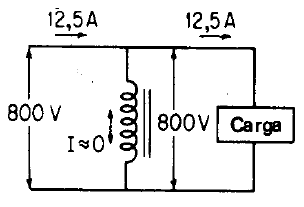
\includegraphics[scale=.4]{relacao11.png}
    \caption{Relação 1:1}
    \label{relacao11}
\end{figure}

As perdas variáveis no cobre do enrolamento do transformador na Figura~\ref{relacao11}
são praticamente nulas, devido à resistência relativamente baixa do enrolamento e à
pequena corrente de excitação. O efeito interessante na regulação do transformadores
é o adição de carga capacitivas, ela estabelece uma ressonância parcial entre a 
reatância indutiva do transformador, de modo, que a tensão secundária tente a aumentar
conforme a carga capacitiva é adicionada.

%%%%%%%%%%%%%%%%%%%%%%%%%%%%%%%%%%%%%%%%%%%%%%%%%%%%%%%%%%%%%%%%%%%%%%%%%%%%%%%%
% carga puramente resistiva
\section{Prática: Carga Resistiva}

A seguinte montagem consiste em um transformador isolado com relação de transformação
1 para 1. Onde no secundário é conectada uma carga puramente resistiva. Antes se faz 
necessário identificar os termos: $V_1$ é a tensão no primário, $I_1$ a corrente 
no primário, $V_2$ a tensão no secundário e $I_2$ a corrente no secundário. O modulo
utilizado foi EMS8341, o primário conectores 1 e 2, secundário 5 e 6, fazendo 
com isso uma relação já dita acima, relação 1:1. A tabela para os diversos valores
foi criada variando apenas a resistência(carga), com isso foi obtida,

\renewcommand{\arraystretch}{1.5}
\begin{center}
    \captionof{table}{} 

    \begin{tabular}{c||c||c||c}
        $R_L$(ohm) & $I_2$(mA) & $E_2$(V) & $I_1$(mA) \\
        \hline
        1200 & 95 & 116.0 & 159 \\
        600 & 174 & 116.0 & 225 \\
        400 & 205 & 114.0 & 305 \\
        300 & 371 & 111.0 & 405 \\
        240 & 456 & 111.0 & 482 \\
    \end{tabular}
\end{center}

\subsection{Calculo da regulação}

A regulação do transformador é o percentual entre tensão do secundário em carga
com a tensão do secundário em vazio, em outras palavras,

\begin{equation}
    Regulacao = \left( \frac{V_{vazio} - V_{carga}}{V_{carga}} \right)*100\%
\end{equation}

Utilizando os valores da Tabela 1 é encontrado os seguintes valores de regulação,

\renewcommand{\arraystretch}{1.5}
\begin{center}
    \captionof{table}{} 

    \begin{tabular}{c||c}
        $R_L$(ohm) & Regulação \\
        \hline
        1200 & 0 $\%$ \\
        600 &  0 $\%$ \\
        400 &  1.7544 $\%$ \\
        300 &  4.5045 $\%$ \\
        240 &  4.5045 $\%$ \\
    \end{tabular}
\end{center}

\subsection{Potência VA}

As potência do primário e secundário são, observação, a tensão no primário
é $116 V$
\renewcommand{\arraystretch}{1.5}
\begin{center}
    \captionof{table}{} 

    \begin{tabular}{c||c||c}
        $R_L$(ohm) & $VA_{primario}$ & $VA_{secundario}$ \\
        \hline
        1200 & 18.44 & 11.02 \\
        600 &  26.10 & 20.18 \\
        400 &  35.38 & 30.21 \\
        300 &  46.98 & 41.18 \\
        240 &  56.35 & 50.62 \\
    \end{tabular}
\end{center}

A comparação da potência do primário e secundário mostra o que já vem
sendo notado com as praticas, o transformador usado apresenta muitas perdas.

%%%%%%%%%%%%%%%%%%%%%%%%%%%%%%%%%%%%%%%%%%%%%%%%%%%%%%%%%%%%%%%%%%%%%%%%%%%%%%%%
% carga Indutiva

\subsection{Experiência: Carga Indutiva}

A mesma experiência feita com a carga resistiva agora é repetida para uma carga
indutiva, os seguintes valores foram medidos,

\renewcommand{\arraystretch}{1.5}
\begin{center}
    \captionof{table}{} 

    \begin{tabular}{c||c||c||c}
        $R_L$(ohm) & $I_2$(mA) & $E_2$(V) & $I_1$(mA) \\
        \hline
        1200 & 109 & 116 & 189 \\
        600 & 196 & 116 & 270 \\
        400 & 300 & 116 & 368 \\
        300 & 325 & 115 & 392 \\
        200 & 510 & 114 & 565 \\
    \end{tabular}
\end{center}

%%%%%%%%%%%%%%%%%%%%%%%%%%%%%%%%%%%%%%%%%%%%%%%%%%%%%%%%%%%%%%%%%%%%%%%%%%%%%%%%
% carga capacitiva

\subsection{Experiência: Carga Capacitiva}

A mesma experiência feita com a carga resistiva agora é repetida para uma carga
capacitiva, os seguintes valores foram medidos,

\renewcommand{\arraystretch}{1.5}
\begin{center}
    \captionof{table}{} 

    \begin{tabular}{c||c||c||c}
        $R_L$(ohm) & $I_2$(mA) & $E_2$(V) & $I_1$(mA) \\
        \hline
        1200 & 117 & 16 & 72 \\
        600 & 248 & 117 & 169 \\
        400 & 358 & 120 & 270 \\
        300 & 462 & 120 & 363 \\
        200 & 580 & 121 & 468 \\
    \end{tabular}
\end{center}

%%%%%%%%%%%%%%%%%%%%%%%%%%%%%%%%%%%%%%%%%%%%%%%%%%%%%%%%%%%%%%%%%%%%%%%%%%%%%%%%
% Conclusão

\section{Conclusão}


\end{document}

